\documentclass[tikz]{standalone}
\usepackage{times}
\usepackage{latexsym}
\usepackage{tabularx}
\usepackage{tikz-qtree}
% BEGIN OWN MODIFICATIONS
\usepackage{amsmath}
\usepackage{amssymb}
\usepackage{arydshln}
\usepackage{booktabs}
\usepackage{tabularx}
\usepackage{tikz}
\usepackage{pgfplots}
\usepackage[normalem]{ulem}
\usepackage{xcolor}
\usepackage{dashbox}%
\usepackage{multirow}
\usepackage{textcomp}
\usepackage{tcolorbox}
\usepackage[ruled, vlined, linesnumbered]{algorithm2e}
\usepackage{mathtools}
\usepackage{soul}
\usetikzlibrary{shadows,arrows.meta,positioning,backgrounds,fit,calc, fadings,shadows,shapes.arrows,intersections}
\pgfplotsset{compat=1.13}


\usetikzlibrary{calc,fit,positioning,arrows}

\renewcommand{\floatpagefraction}{.8}%TODO remove this for the final version
\newcommand{\bftab}{\fontseries{b}\selectfont}
\newcommand\mask{\_\_\_}

\pgfdeclarelayer{bg}    % declare background layer
\pgfsetlayers{bg,main}  % set the order of the layers (main is the standard layer)
\definecolor{plot1}{RGB}{243,96,157}
\definecolor{plot2}{RGB}{157,210,255}
\definecolor{plot3}{RGB}{125,167,125}
\definecolor{plot4}{RGB}{247,147,29}
\definecolor{plot5}{RGB}{230,150,50}
\definecolor{plot6}{RGB}{130,67,34}
\definecolor{plot7}{RGB}{230,167,134}
\definecolor{decentgrey}{RGB}{167,167,172}

\begin{document}


\begin{tikzpicture}
\def\tmspacing{0.8cm}
\def\mtspacing{1.6cm}
\def\dspacing{0.2cm}


\begin{axis}[legend style={nodes={scale=0.6, transform shape}}, 
cycle list name=color list,
xlabel={$\lambda$},
ylabel={macro F1 score (\%)},
ymin = 60,
ymax = 90,
xmin = 0,
xmax = 8,
enlarge x limits={0.075},
enlarge y limits={0.075},
xtick = {1, 2, 3, 4, 5, 6, 7, 8},
xticklabels = {0, 0.1, 0.2,1,2,5,10},
xtick pos=left,
ytick pos=left,
ylabel near ticks,
xlabel near ticks,
tick align=outside,
major tick length=0.075cm,
width = 0.85\linewidth,
height = 0.2\textheight,
x tick label style={/pgf/number format/1000 sep=},
legend image post style={scale=0.4},
legend style={draw=decentgrey, at={(0.98,0.05)},anchor=south east, font=\footnotesize},
legend cell align=left,
legend columns=1,
tick label style={font=\footnotesize}
]        
\addplot[mark=*, thick, plot5] coordinates {
(0,80.4)
(1,82.4)
(2,81.1)
(3,86.4)
(4,79.4)
(5,78.4)
(6,82.1)
(7,80.6)
};
\end{axis}

\end{tikzpicture}
\end{document}